\textit{Cette partie présente \emph{Hibernate}, l'ORM que nous avons du utiliser pour gérer l'accès aux données. Elle détaille également les différents paquets de l'application, la manière dont ont été mappé les informations, celle adoptée pour la génération du graphe, ainsi que l'utilisation de l'outil développé en ligne de commande. Notons que l'utilisation du langage Java ne sera pas justifié étant donné qu'il s'agit d'une contrainte induite pas le fait que le framework \emph{Hibernate} devait être utilisé.}

\section{L'ORM \emph{Hibernate}}
\emph{Hibernate} est un framework Java de type ORM. Bien qu'il permette la gestion de la persistance des données (écriture), \emph{Hibernate} sera utilisé ici uniquement dans le but d'accéder aux métadonnées des SGBD (lecture) via des configurations de Mapping.
\subsection{POJO}
La définition des entités dans \emph{Hibernate} à l'aide de classes \emph{POJO}. Cet acronyme signifiant \og Plain Old Java Object \fg{} fait référence à de simples classes ayant comme principale caractéristique de n'implémenter aucune interface, et de posséder un \emph{getter} et un \emph{setter} par attribut.
\subsection{Mapping}
Le mapping consiste, comme son nom l'indique, à faire la correspondance entre les entités définies (classes \emph{POJO}) et les tables en base de données. En règle générale, un objet $x$ est mappé avec une table relationnelle $table-x$, est les attributs $x_1$, $x_2$, \ldots, $x_n$ avec les attributs $tables-x.x_1$, $tables-x.x_1$, \ldots, $tables-x.x_1$. Il est également possible d'ajouter des relations entre attributs (One-to-One, One-to-Many, Many-to-Many), de déclarer des \emph{id}, etc.

\emph{Hibernate} permet de définir le mapping via des annotations directement au sein des classes, ou via des fichiers de configuration xml \texttt{hbm}. C'est cette deuxième méthode que nous avons choisie, et qui sera décrite dans la partie~\ref{section:structure_de_lapplication}.
\subsection{Subselect}

\subparagraph{\ldots}

\section{Structure de l'application}
\label{section:structure_de_lapplication}

Dans le but de faciliter la réutilisation du code et l'extension de sa compatibilité avec de nouveaux SGBDR, nous avons pris soin de structurer l'application. La figure~\ref{figure:structure_appli} présente l'arborescence des paquets Java.

\begin{figure}[H]
\centering
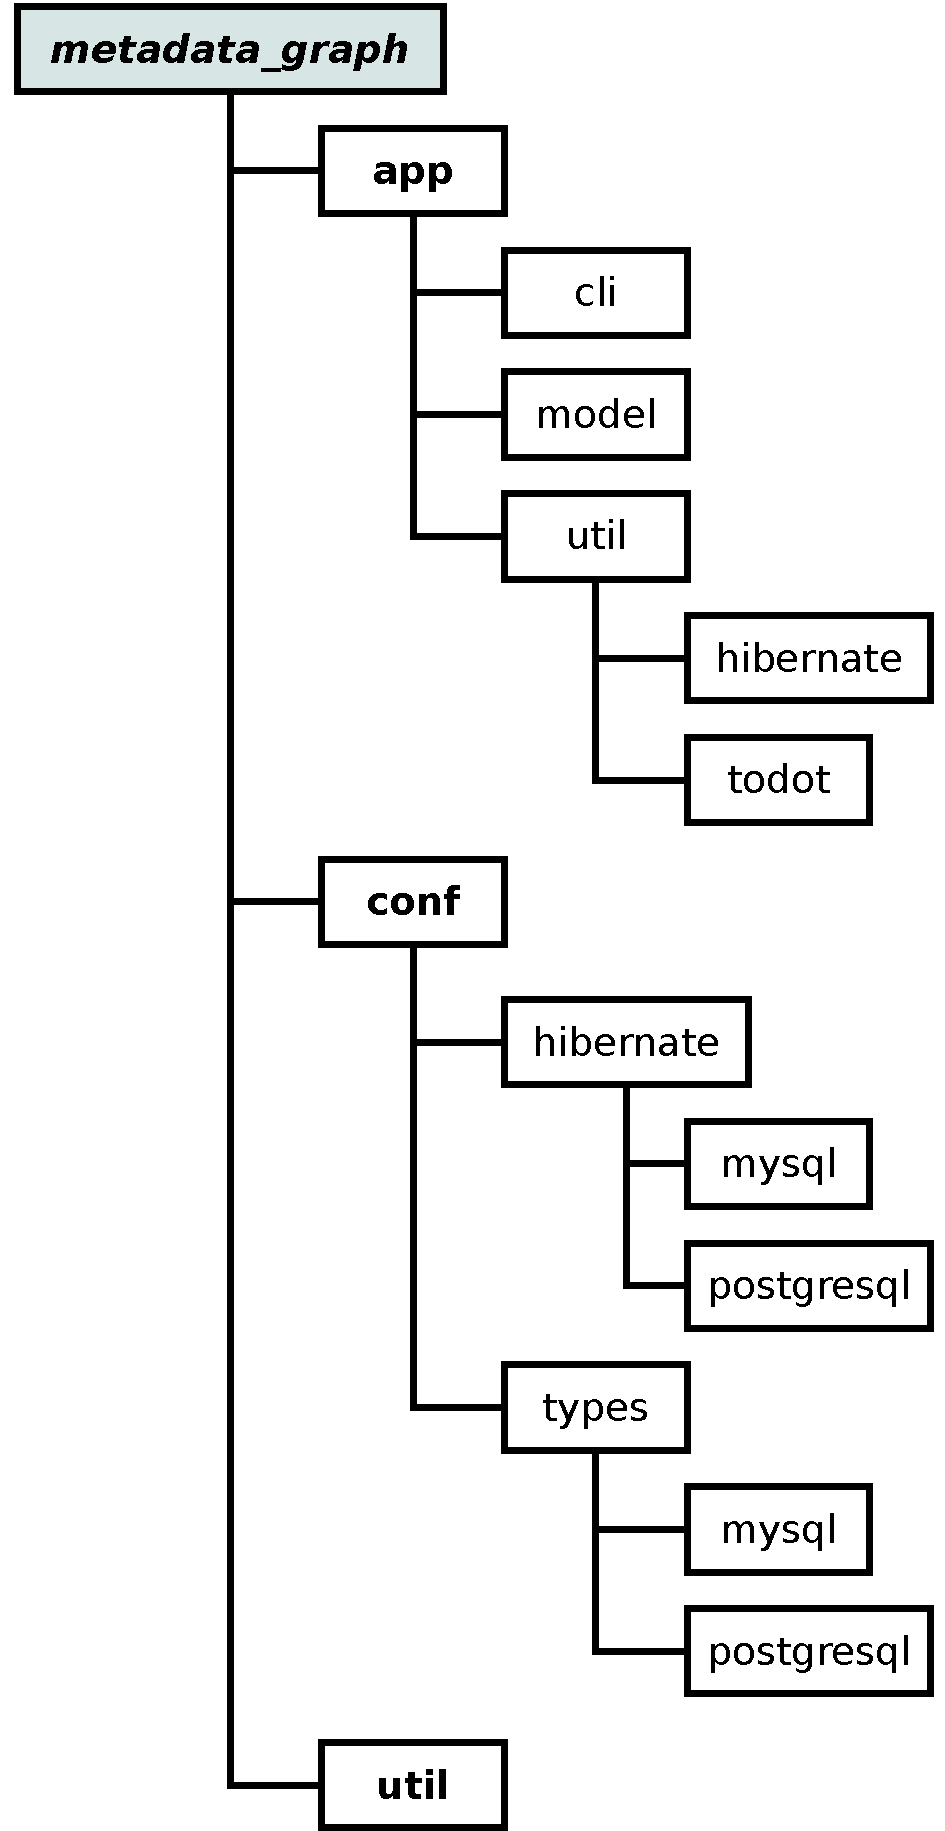
\includegraphics[width=0.5\textwidth]{files/archi}
\caption{Arborescence des paquets Java de l'application.}
\label{figure:structure_appli}
\end{figure}

Trois paquets principaux se distinguent :

\begin{description}
\item[\texttt{app}] : dans ce paquet sont regroupés toutes les classes Java nécessaires au fonctionnement interne de l'outil. On y trouve les sous paquets \texttt{cli}, \texttt{model} et \texttt{util} qui seront détaillés par la suite.
\item[\texttt{conf}] : ce paquet permet d'externaliser les fichiers de configuration. Il a la particularité de ne stocker aucune classe Java.
\item[\texttt{util}] : ici sont regroupés des classes java utilisées par l'application mais qui ne sont pas propre à l'exécution de ses fonctions initiales. Elle stocke notamment des classes permettant la gestion du CLI.
\end{description}

\subsection{Paquet \texttt{app.cli}}

Ce paquet implémente l'interface en ligne de commande, celle-ci permettra notamment la configuration de la connexion au SGBDR ainsi que le format de sortie. Il est composé exclusivement de la classe \texttt{CommandLineInterface}.

\begin{description}
\item[CommandLineInterface] Cette classe défini la fonction \texttt{main} de notre application. Elle utilise la classe \texttt{OptionManager} décrite en \ref{subsection:util} page \pageref{subsection:util} afin d'interpréter les options de la ligne de commande.  
\end{description}

\begin{verbatim}
Usage:
gd SGBD_NAME DATABASE_NAME [OPTION]...

Options:
    -u, --user <USERNAME>
        use this username.
    -p, --password [PASSWORD]
        use this password.
    -h, --host <HOST>
        use this host.
    --port <PORT>
        use this port.
    -o, --output <FILE_NAME>
        generate a png image with graphviz
    -T, --type <type>
        the output format : svg, ps, png, gif, dia… 
        See graphviz output formats for more formats.
    -c, --cmd <GRAPHVIZ_CMD>
        choose your graphviz command (man graphviz).
    --show 
        open a window with graph representation.
    --help
        print this message.
\end{verbatim}


\subsection{Paquet \texttt{app.model}}
C'est ici que sont définies les classes \emph{POJO} du modèle de données correspondant au modèle relationnel. On y trouve donc les classes \texttt{Column}, \texttt{Constraint} et \texttt{Table}, enrichies de quelques méthodes :

\begin{description}

\item[Column] Ajout d'un méthode \texttt{\underline{bool isPk()}} permettant de savoir si la colonne est inclue dans la clé primaire de la table à laquelle elle appartient. Est également définie une méthode \texttt{\underline{String getGenericType()}} qui retourne, sous la forme d'une chaine de caractères, le type générique de la colonne.

\item[Constraint] Ajout des méthodes \texttt{\underline{bool isPk()}}, \texttt{\underline{bool isFk()}} et \texttt{\underline{bool isCheck()}} permettant de savoir respectivement si la contrainte est de type clé primaire, clé étrangère, ou contrainte de vérification. Est également définie une méthode \texttt{\underline{String getGenericType()}} qui retourne, sous la forme d'une chaine de caractères, le type générique de la contrainte.
\end{description}

Les types génériques sont définies dans les énumérations \texttt{ColumnType} et \texttt{ConstraintType}. Les conversions de types se font en fonction du SGBDR sélectionné grâce au paquet \texttt{app.util} (cf. \ref{subsection:app.util}) et aux fichiers de conversions stockés dans le paquet \texttt{conf.types} (cf. \ref{subsection:conf.types}).

\subsection{Paquet \texttt{app.util}}
\label{subsection:app.util}

Des classes utilitaires sont définies dans ce paquet.

\subsubsection{Génération de graphe avec \texttt{ToDotUtil}}
\label{section:ToDotUtil}
Cet utilitaire est définit dans un sous paquet \texttt{todot}. Il contient une succession d'énumérations permettant de lister les commandes \emph{graphviz}, les couleurs, les formes, et les styles propres au langage DOT.
La classe principale \texttt{ToDotUtil} implémente une méthode permettant, à partir d'une base de données (liste de tables), de générer une chaine de caractères au langage DOT qui décrit cette base de données. Il est possible de définir le style du graphe généré en sortie (couleurs, formes, etc.).

Les formats d'exportation suivant sont reconnus : 

\begin{center}
\begin{tabular}{c c c c c c}
canon&cmap&cmapx&cmapx\_np&dot&eps \\
fig & gd & gd2 & gif & gv & imap \\
imap\_np & ismap & jpe & jpeg & jpg & pdf \\
plain & plain-ext & png & ps & ps2 & svg \\
svgz & tk & vml & vmlz & vrml & wbmp \\
x11 & xdot & xlib & & & \\
\end{tabular}
\end{center}

\subsubsection{Singleton de connexion Hibernate}
Le sous paquet \texttt{hibernate} contient une classe \texttt{HibernateUtil} respectant le patron de conception \emph{singleton}. Il permet de créer une session \emph{Hibernate} en fournissant le type de SGBD, l'hôte, le nom de la base de données, le nom d'utilisateur, le mot de passe et le port.

La création de la session s'effectue en chargeant le fichier de configuration \emph{Hibernate} correspondant au type de SGBD passé en paramètre, et renvoie une exception si celui-ci est inexistant ou inaccessible.

\subsubsection{Types génériques}
Comme décrit dans la section~\ref{section:generic_types}, nous avons fait le choix de généraliser les types de colonnes et de contraintes. Cette classe utilitaire fournit une unique méthode permettant, à partir du type de SGBD, du type non générique, et du type d'objet (colonne ou contrainte), de retourner le type générique. La méthode procède en chargeant le fichier de correspondance des types du SGBD passé en paramètre. Ces fichiers sont décrits dans la section~\ref{subsection:conf.types}.

\subsection{Paquet \texttt{conf.hibernate}}
Les fichiers de configurations d'\emph{Hibernate} propre à chaque SGBDR sont stockés ici. Il faut créer un sous paquet au nom du SGBDR (en respectant le nom du driver JDBC).

Chaque SGBDR doit posséder quatre fichiers de configuration. La configuration principale déclare le driver et le dialecte à utiliser, ainsi que les chemin vers les trois fichiers de Mapping décrits ci-après.
\subsubsection{Fichiers de mapping}
\paragraph{Le \emph{subselect}} Le subselect permet d'associer non pas une entité du modèle à une table réellement stockée en  base de données, mais à un table virtuelle créée via un requête de sélection. Nous avons donc pu généraliser notre modèle de données en adaptant les clauses \emph{subselect} pour chaque SGBD, afin de sélectionner, à partir des vues proposées par les différents systèmes, les données nécessaires.

\paragraph{Problématique de la relation \emph{Many-to-Many}}
Lors de la construction de nos fichiers de mapping, nous avons rencontré un problème au niveau du modèle de données auquel nous étions confrontés (cf. figure~\ref{figure:diag_classe_reel}, page \pageref{figure:diag_classe_reel}). D'après ce modèle, l'entité contrainte est en relation \emph{Many-to-Many} avec l'entité colonne. Dans le modèle relationnel, une telle relation nécessite la création d'une table d'association, permettant la jointure entre ces deux entités. Étant donné que nous travaillons avec des \emph{subselect}, nous ne pouvons pas créer de telle table. La solution a donc consisté en adaptant le schéma réel afin de pallier à cet imprévu.

L'idée est donc de transformer cette relation problématique en une relation \emph{Many-to-One} (plusieurs relations peuvent être en relation avec une seule colonne). Pour cela, il faut utiliser des id composés (\emph{composite-id}) en identifiant une contrainte non plus uniquement pas sa table et son nom, mais pas sa table, son nom, et le nom de la colonne. Ainsi, une contrainte s'appliquant sur deux colonnes sera représentée par deux instances de la classe contrainte.

\begin{figure}[H]
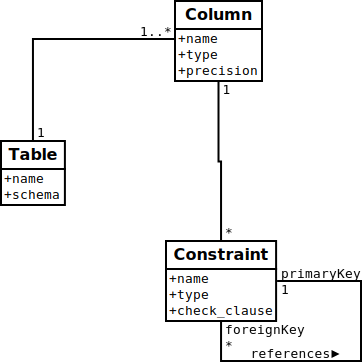
\includegraphics[width=0.6\textwidth]{files/diag_class_final}
\centering
\caption{Diagramme de classe représentant le modèle \emph{Hibernate}.}
\label{figure:diag_class_model_hibernate}
\end{figure}

\subsection{Paquet \texttt{conf.types}}
\label{subsection:conf.types}

Les types génériques sont définis dans des fichiers xml placés dans des sous paquets. A chaque type générique définis dans l'application, il suffit d'associer les types réels propres au SGBDR. 

Voici la DTD de ces fichiers de correspondance : 
\begin{verbatim}
<!ELEMENT genericTypes (genericType*)>
<!ELEMENT genericType (type*)>
<!ELEMENT type (#PCDATA) >

<!ATTLIST genericType name CDATA #REQUIRED>
\end{verbatim}


\subsection{Paquet \texttt{util}}
\label{subsection:util}

Dans ce paquet sont regroupé toutes les classes utilitaires non spécifique à l'application. 

\begin{description}
\item[OptionManager] Cette classe aide à la gestion des paramètres passé à une application.

\item[ImageFrame] Permet d'ouvrir facilement une fenêtre contenant une image.

\item[XmlUtil] Fournit une méthode pour parser des fichiers XML.
\end{description}

